% !TEX program = xelatex
\documentclass[10pt, aspectratio=169]{beamer}
% [인쇄/배포할 때] -> 이 줄을 활성화하세요
%\documentclass[handout, aspectratio=169]{beamer}
\usefonttheme{professionalfonts}
\usepackage{totcount}   % 전체 카운터 계산 패키지
\regtotcounter{section} % 섹션의 전체 개수를 세도록 등록
\usetheme{metropolis}
% 숨겨진 텍스트를 완전히 지우지 않고 15% 농도로 흐릿하게 보여줌
\setbeamercovered{transparent}
\metroset{sectionpage=progressbar, progressbar=frametitle}


\usepackage{pgfplots}
\pgfplotsset{compat=1.18}
\usepgfplotslibrary{fillbetween}
\usepackage{graphicx, caption, hyperref, fontawesome5}
\usepackage{subcaption}
\usepackage{cleveref} % hyperref보다 나중에 불러와야 함
\usepackage{ulem} % 밑줄 긋기 (취소선 등)
\usepackage{lipsum} % 더미 텍스트 생성
\usepackage{fancybox, tcolorbox} % 박스 생성
\usepackage{tcolorbox}  % 박스 생성
\tcbuselibrary{skins, breakable, theorems, many}   % 박스 스킨 라이브러리
\usepackage{multicol} % 다중 컬럼 환경
\usepackage{multirow} % 셀 병합 기능
\usepackage{booktabs} % 예쁜 가로선 (\toprule, \midrule, \cmidrule, \bottomrule)}
\usepackage{refcount} % 참조된 라벨의 번호 가져오기
% [수식 및 폰트 설정 - 기존 파일 그대로 유지]
\usepackage{amsmath}
\usepackage{mathtools}
\usepackage[math-style=ISO, bold-style=ISO]{unicode-math}
\usepackage{array}
\usepackage{enumitem}
\usepackage{xcolor}
\usepackage{tikz}
\usetikzlibrary{positioning, shapes.geometric, arrows.meta, calc, fit, backgrounds, shapes.geometric, shadows.blur, shapes.symbols, decorations.pathmorphing, decorations.text, 3d, patterns, plotmarks}

\usetheme{metropolis}

% --- [1. 색상 및 스타일 정의] ---
\definecolor{proBlue}{HTML}{4477AA}  
\definecolor{hiOrange}{HTML}{DDAA33} 
\definecolor{mythRed}{HTML}{B22222}
\definecolor{factGreen}{HTML}{228B22}

% --- [디자인 포인트: 00_blockchain_orientation 스타일 반영] ---
\definecolor{proBlue}{HTML}{4477AA}   % 메인 테마 블루
\definecolor{hiOrange}{HTML}{DDAA33}  % 포인트 골드/오렌지
\definecolor{ethPurple}{HTML}{454A75} % 보조 컬러
% ---------- Metropolis colour tweaks ----------
\definecolor{mBlue}{RGB}{0,82,147}
\definecolor{mOrange}{RGB}{230,110,0}
\definecolor{mGreen}{RGB}{0,140,80}
\definecolor{mRed}{RGB}{180,30,30}
\setbeamercolor{frametitle}{bg=mBlue}
\setbeamercolor{progress bar}{fg=mOrange}
\setbeamercolor{alerted text}{fg=mOrange}

% #
%\setbeamercolor{frametitle}{bg=proBlue, fg=white}
\metroset{sectionpage=progressbar, progressbar=frametitle}

% --- [2. 필수 패키지 및 라이브러리] ---
\usepackage{kotex}

% --- [3. 폰트 설정] ---
\usepackage{fontspec}
\setmainfont{FiraSans-Regular.ttf}[Path = ../../fonts/, BoldFont = FiraSans-Bold.ttf]
\setsansfont{FiraSans-Regular.ttf}[Path = ../../fonts/, BoldFont = FiraSans-Bold.ttf]
\setmainhangulfont{NotoSansKR-Regular.ttf}[Path = ../../fonts/, BoldFont = NotoSansKR-Bold.ttf]
\setsanshangulfont{NotoSansKR-Regular.ttf}[Path = ../../fonts/, BoldFont = NotoSansKR-Bold.ttf]

\graphicspath{
    {./}
    {../../99_Assets/}
    {../../99_Assets/images/}
}

% 기존 설정이 있다면 아래와 같이 변경합니다.
\metroset{
  sectionpage=none,    % 섹션 간지 생성 중지
  progressbar=frametitle
}

% --- [4. 교수님 정보 설정] ---
\author{
    이 경 근 \\
    {\tiny
        % \texorpdfstring{문서에 보일 내용}{PDF 속성에 들어갈 텍스트(특수문자 제외)}
        \texorpdfstring{\raisebox{-0.1ex}{\scalebox{0.85}{\faEnvelope}}}{} \href{mailto:infosec@knu.ac.kr}{infosec@knu.ac.kr} \quad 
        \texorpdfstring{\scalebox{0.9}{\faLinkedin}}{} \scalebox{0.9}{\href{https://www.linkedin.com/in/Kenny-0633-Lee}{Kenny-0633-Lee}}
    }
}
\institute{ABB -- DNA -- KNU}
\title{Blockchain Technology and Applications}
\subtitle{Building Trust without Intermediaries}
\date{Spring 2026}


%%%%%%%%%%%%%%%%%%%%%%%%%%%%%%%%%%%%%%%%%%%%%%%%%%%%%%%%
%%%%%%%%%%%%%%%%%%%%%%%%%%%%%%%%%%%%%%%%%%%%%%%%%%%%%%%%
%%%%%%%%%%%%%%%%%%%%%%%%%%%%%%%%%%%%%%%%%%%%%%%%%%%%%%%%
\begin{document}

% Slide 1: Title
\begin{frame}[plain]
    \titlepage
\end{frame}



% Slide 2: Opening - Live Blockchain Ecosystem (mempool.space)
\section{Live Ecosystem}
\begin{frame}{Opening: mempool.space}
    \centering
    \vspace{-0.2cm}
    
    % 1. 메인 스크린샷 이미지
%    \IfFileExists{fig_ch00_mempool_big.png}{
        \begin{tcolorbox}[colframe=proBlue!20, colback=white, boxrule=0.5pt, arc=3pt, boxsep=0pt, left=2pt, right=2pt, top=2pt, bottom=2pt]
            \centering
            % 파일명 안의 언더바(_)는 인클루드 시 그대로 적습니다.
            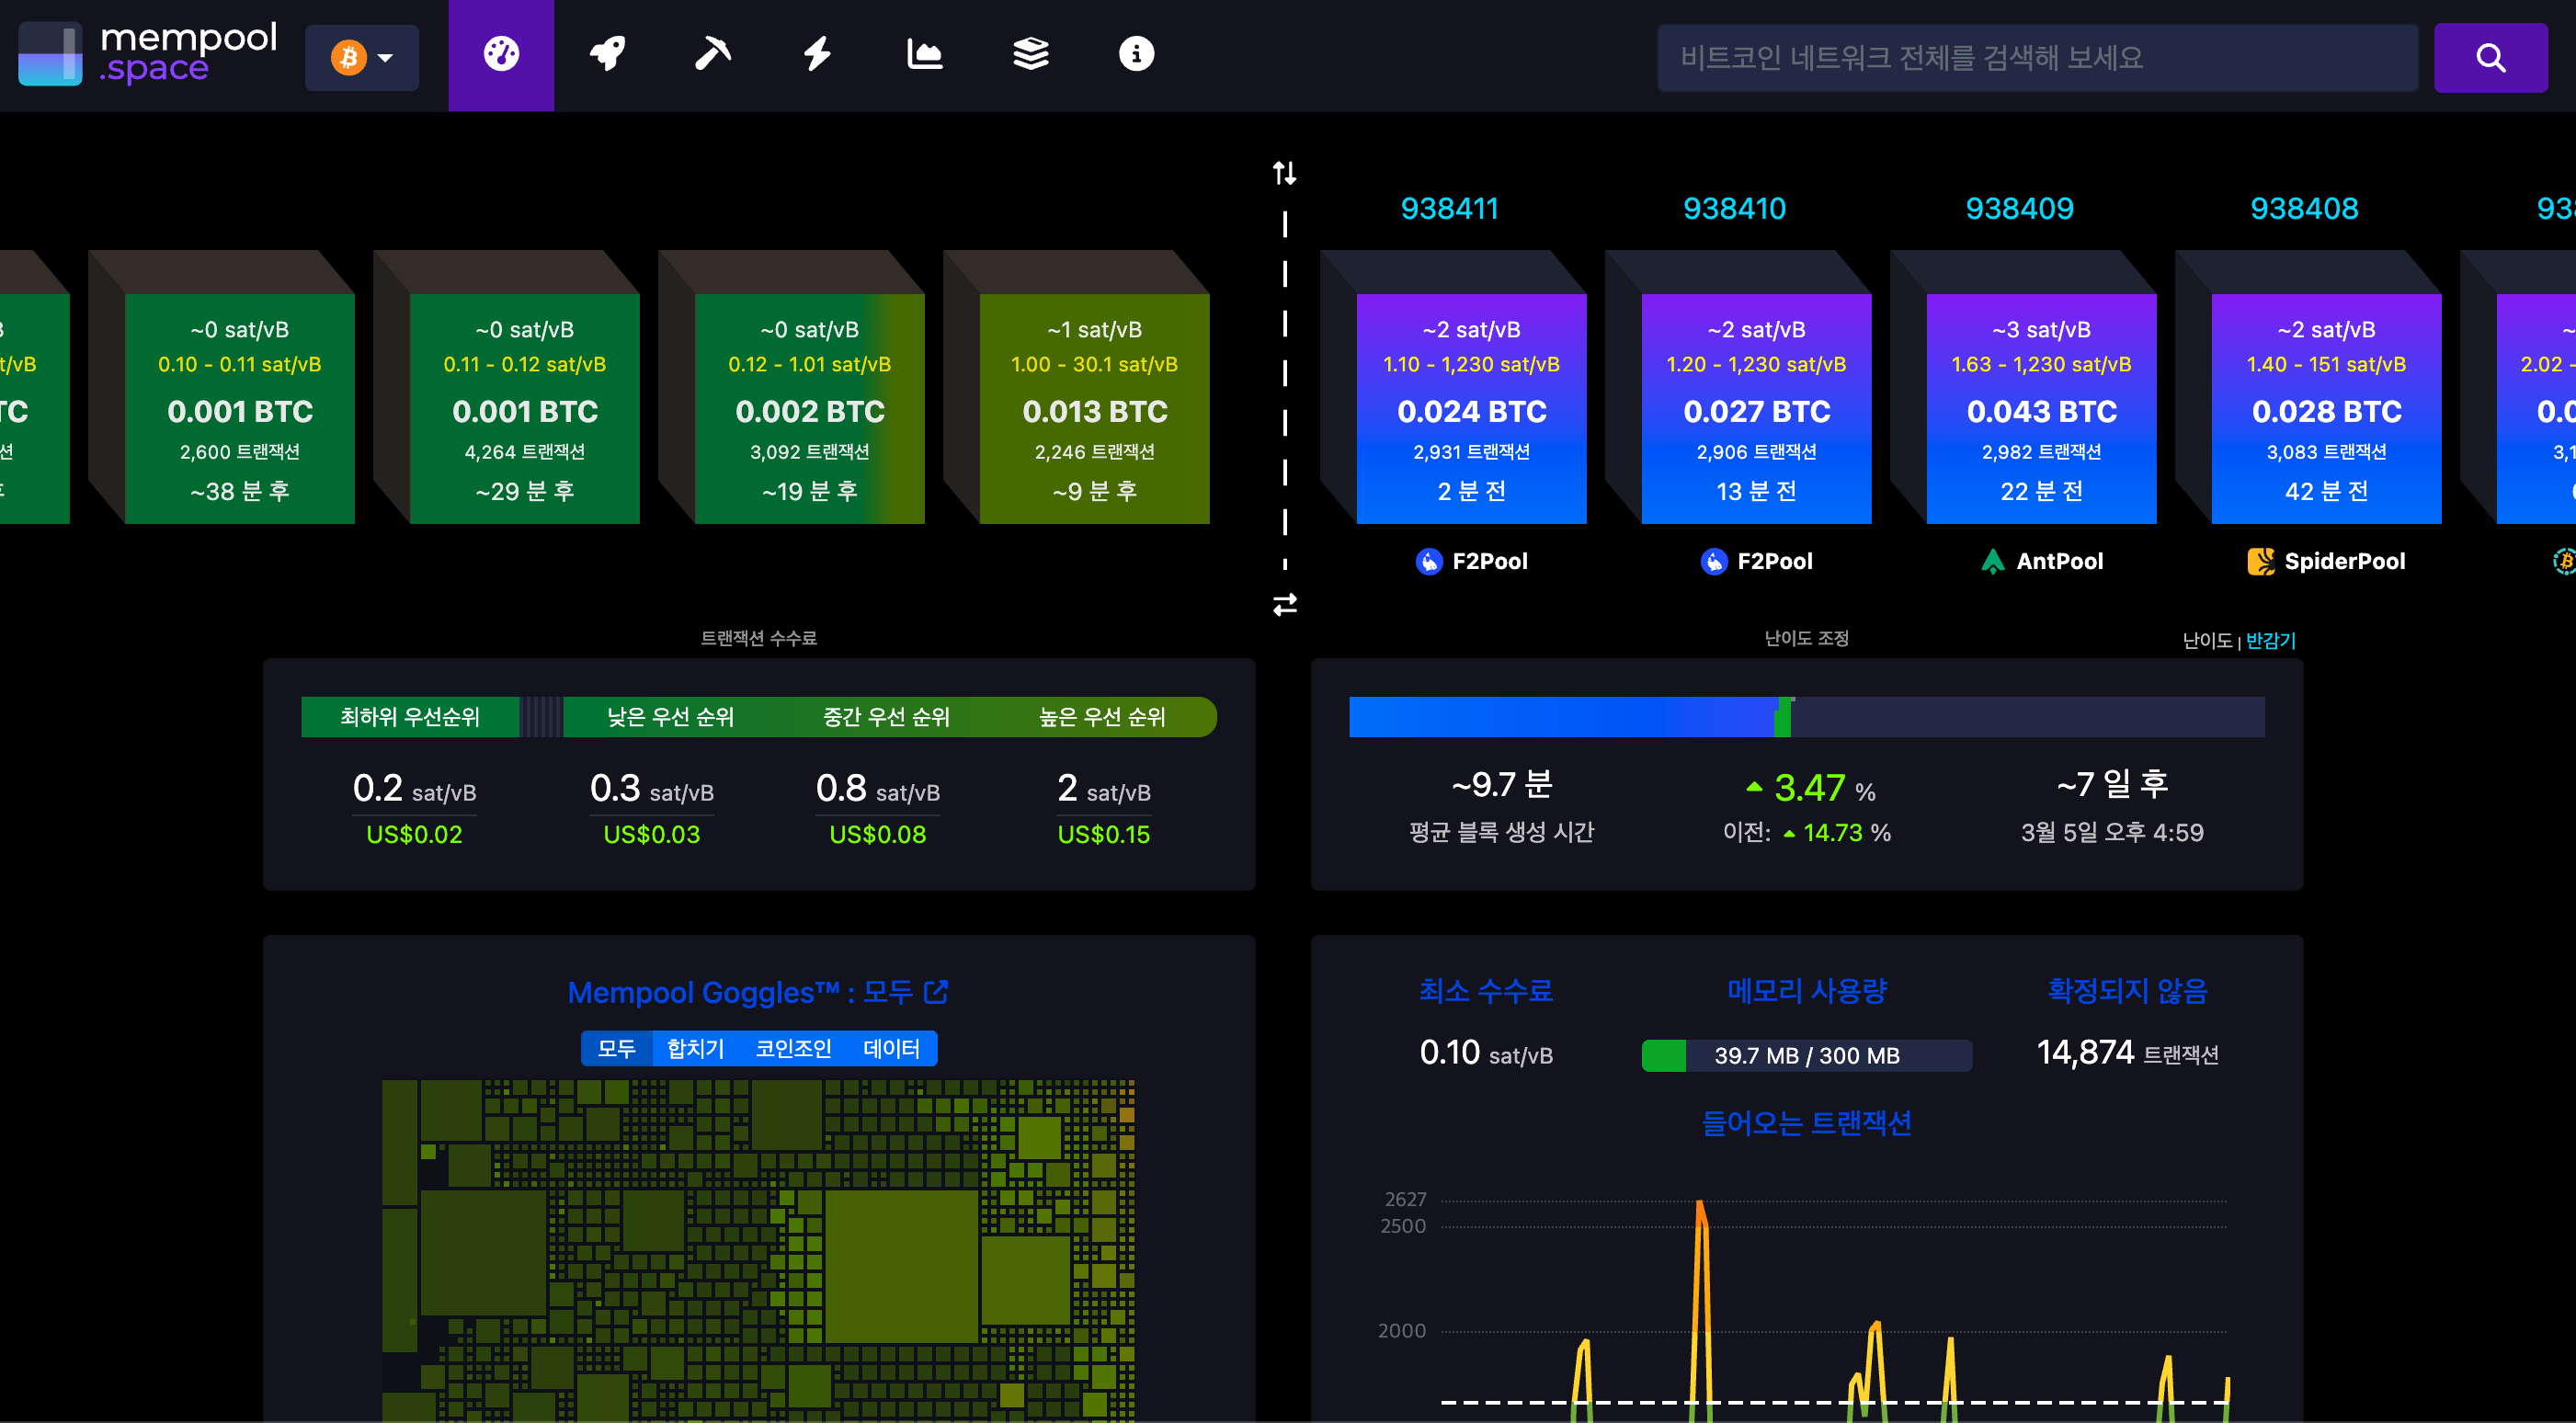
\includegraphics[width=0.92\textwidth, height=0.72\textheight, keepaspectratio]{fig_ch00_mempool_big.png}
        \end{tcolorbox}
 %   }{
    %     % 파일이 없을 경우의 TikZ 가이드 (에러 수정 완료)
    %     \begin{tikzpicture}
    %         \draw[draw=gray!50, fill=gray!5, dashed, thick] (0,0) rectangle (12, 5.5) 
    %         node[pos=.5, align=center, font=\small, color=gray] {
    %             \faImage \\ \relax [fig\_ch00\_mempool\_big.png] 이미지를 넣어주세요 \\ 
    %             (화면 과반 이상 점유 설정 완료)
    %         };
    %     \end{tikzpicture}
    % }

    \vfill
    
    % 2. 라이브 사이트 링크
    {\small \faLink~~ \href{https://mempool.space/ko/}{\color{proBlue}\textbf{mempool.space/ko/}} : Visualizing a Bitcoin node's mempool as projected blocks}
\end{frame}



% Slide 3: What is Blockchain? (The Three Pillars)
\section{Definition}
\begin{frame}{What is Blockchain? (The Three Pillars)}
    \begin{columns}
        \begin{column}{0.45\textwidth}
            \centering
            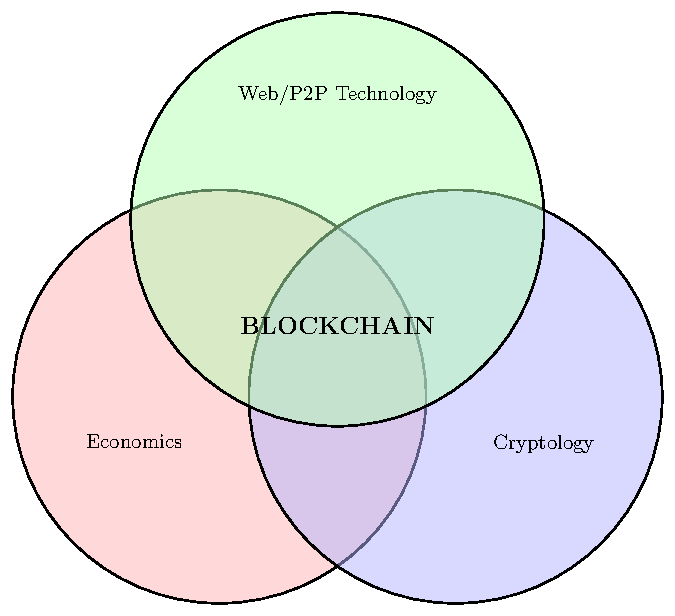
\includegraphics[width=0.85\textwidth]{venn.pdf}
            \vspace{0.2cm}
            \scriptsize \textbf{Blockchain 3대 핵심 요소}
        \end{column}
        \begin{column}{0.55\textwidth}
            \small
            \begin{itemize}
                \item \textbf{Web/P2P Tech}: 중앙 서버 없는 분산 네트워크.
                \item \textbf{Cryptology}: 무결성을 보장하는 암호학적 기법.
                \item \textbf{Economics}: 네트워크 유지를 위한 게임 이론.
            \end{itemize}
            \begin{tcolorbox}[colback=proBlue!5, colframe=proBlue, boxrule=0.5pt, sharp corners]
                \tiny 세 요소의 교집합이 만드는 \textbf{'신뢰 프로토콜'}.
            \end{tcolorbox}
        \end{column}
    \end{columns}
\end{frame}


% Slide 4: Common Misconceptions vs. Hard Truths
\begin{frame}{Common Misconceptions vs. Hard Truths}
    \begin{columns}
        % 왼쪽: 정부 문서 이미지 영역
        \begin{column}{0.5\textwidth}
            \begin{tcolorbox}[
                title=\faFileContract ~ 블록체인을 잘못 이해한 사례, 
                colframe=proBlue!80,
                colback=white,
                after upper={\par\vspace{0.2cm}\centering\scriptsize \color{gray} [그림1] 과학기술정보통신부의 4차 산업혁명 블록체인 발전전략 문서}
            ]
                \centering
                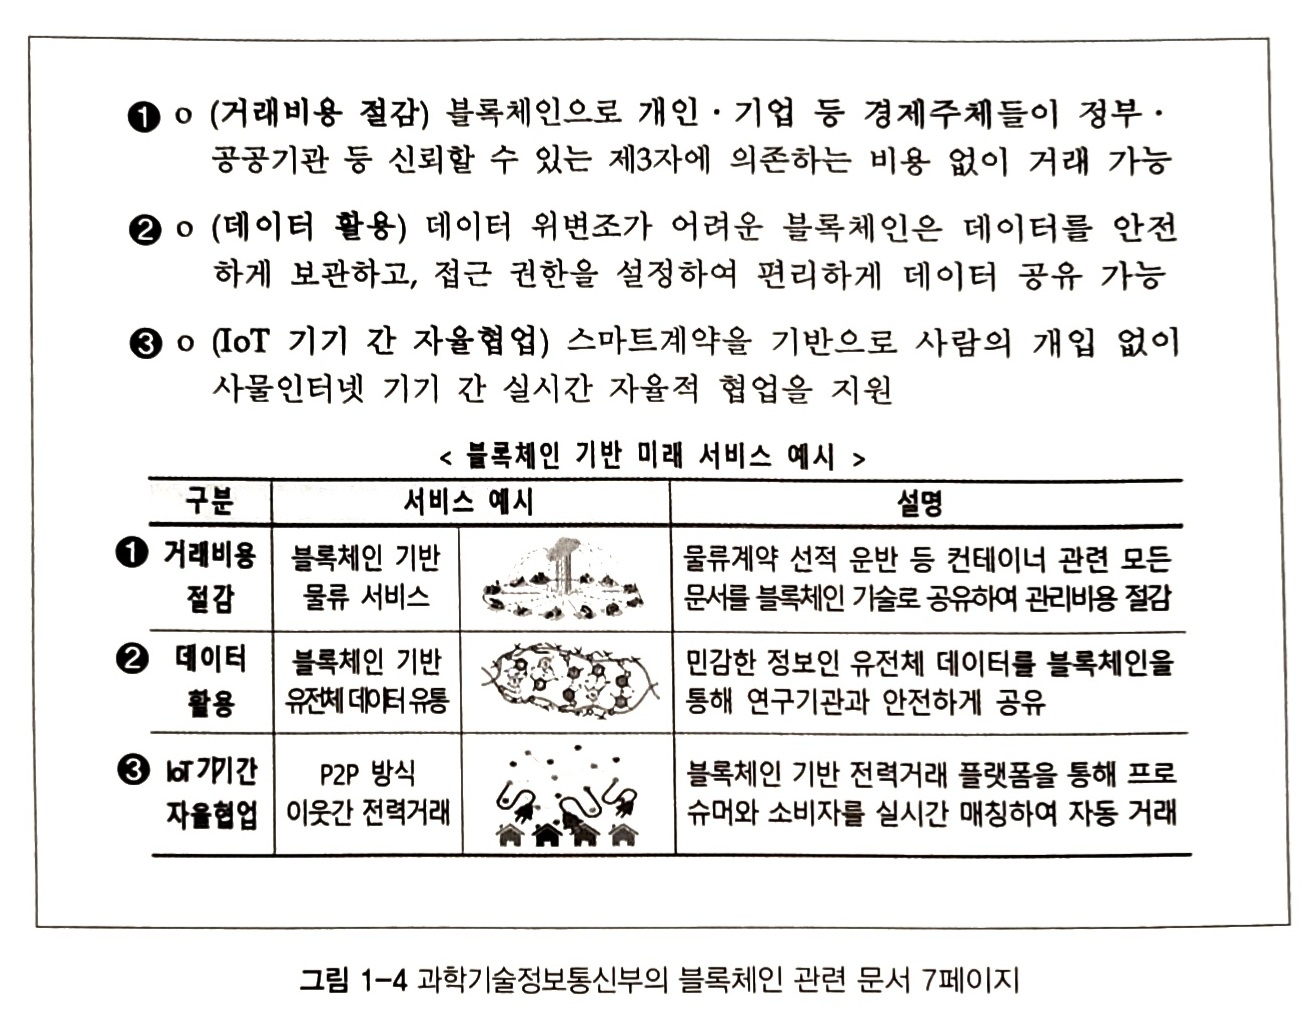
\includegraphics[width=\textwidth, height=4.5cm, keepaspectratio]{fig_ch00_mis_perception.jpg}
            \end{tcolorbox}
        \end{column}

        % 오른쪽: 상세 분석 내용 (밀도를 높여서 보강)
        \begin{column}{0.48\textwidth}
            \small
            \begin{itemize}
                \item \textbf{\color{mythRed}Myth 1. ``거래비용 절감?''}
                \begin{itemize}
                    \item \scriptsize 공공기관이 운영하더라도 노드 유지비용은 발생함. \textbf{신뢰 비용의 구조적 재배치}가 본질.
                \end{itemize}
                \vspace{0.2cm}
                \item \textbf{\color{mythRed}Myth 2. ``데이터를 안전하게 보관?''}
                \begin{itemize}
                    \item \scriptsize '블록체인은 거대한 DB'라는 오해. 실제 데이터는 \textbf{Off-chain}에, 위변조 검증용 \textbf{해시(Hash)}만 기록.
                \end{itemize}
                \vspace{0.2cm}
                \item \textbf{\color{mythRed}Myth 3. ``IoT 기기간 자율 협업?''}
                \begin{itemize}
                    \item \scriptsize 블록체인 자체로 IoT 기기간 지능형 통신을 지원하지는 않음. 오히려 코드가 집행력을 가지는 \textbf{Active Infrastructure}로서의 가치.
                \end{itemize}
            \end{itemize}
        \end{column}
    \end{columns}
\end{frame}


% Slide 5: DID & Mobile ID
\section{Real-world Tech}
\begin{frame}{Standard: DID \& Mobile Driver's License}
    \centering
    
    \begin{tikzpicture}[node distance=1.5cm, box/.style={rectangle, draw=proBlue, fill=white, thick, minimum width=2.2cm, minimum height=1cm, align=center, font=\scriptsize\bfseries}]
        \node[box] (Issuer) {Issuer\\(경찰청)};
        \node[box, right=1.5cm of Issuer] (Holder) {\faMobile*\\Holder\\(지갑)};
        \node[box, right=1.5cm of Holder] (Verifier) {Verifier\\(검증자)};
        \node[box, below=0.8cm of Holder, dashed, draw=gray] (BC) {\faLink\ Blockchain};
        
        \draw[->, thick, proBlue] (Issuer) -- (Holder) node[midway, above, font=\tiny] {VC 발급};
        \draw[->, thick, proBlue] (Holder) -- (Verifier) node[midway, above, font=\tiny] {VP 제출};
        \draw[->, dashed, gray] (Verifier) |- (BC) node[pos=0.75, right, font=\tiny] {상태 검증};
    \end{tikzpicture}
    \vspace{0.2cm}
    \begin{columns}[T]
        \begin{column}{0.65\textwidth}
            \scriptsize
            \textbullet\ \textbf{SSI (자기주권 신원)}: 개인 데이터의 주권 확보. \\
            \textbullet\ \textbf{ZKP (영지식 증명)}: 정보 노출 없는 증명 기술.
        \end{column}
        \begin{column}{0.35\textwidth}
            \begin{tcolorbox}[colback=hiOrange!5, colframe=hiOrange, boxrule=0.5pt]
                \tiny \textbf{Message:} 블록체인 $\neq$ 코인. \\ 우리 일상의 \textbf{보안 표준}입니다.
            \end{tcolorbox}
        \end{column}
    \end{columns}
\end{frame}

% --- [추가 슬라이드 5-1: DID 표준 및 모바일 신분증 흐름] ---
\begin{frame}{DID Standard: Mobile ID \& VC Flow}
    \begin{columns}
        % 왼쪽: 운전면허증 샘플 이미지 및 설명
        \begin{column}{0.4\textwidth}
            \begin{tcolorbox}[title=\faIdCard ~ Mobile Driver's License, colframe=proBlue]
                \centering
                % 실제 이미지 파일이 있다면 파일명으로 교체하세요
                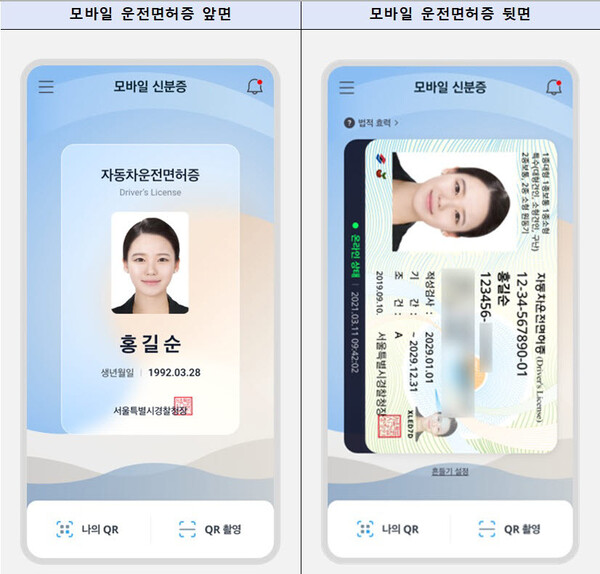
\includegraphics[width=0.8\textwidth]{fig_ch00_driver_license.jpg} \\
                \vspace{0.2cm}
                \footnotesize \color{gray} [국가 모바일 운전면허증 샘플]
            \end{tcolorbox}
            \scriptsize
            \begin{itemize}
                \item \textbf{Privacy:} 필요한 정보(성인 여부 등)만 선택적 제출
                \item \textbf{Security:} 블록체인 기반 위변조 방지
            \end{itemize}
        \end{column}

        % 오른쪽: VC 흐름도 (TikZ로 구현)
        \begin{column}{0.55\textwidth}
            \centering
            \textbf{\small VC (Verifiable Credential) Lifecycle} \\
            \vspace{0.3cm}
            \begin{tikzpicture}[node distance=1.5cm, every node/.style={fill=white, font=\sffamily\tiny}, align=center]
                % Nodes
                \node (issuer) [draw, rectangle, rounded corners, fill=proBlue!10] {\faUniversity\\**Issuer**\\(경찰청/도로교통공단)};
                \node (holder) [below=of issuer, draw, rectangle, rounded corners, fill=hiOrange!10] {\faUserSecret\\**Holder**\\(사용자/전자지갑)};
                \node (verifier) [right=of holder, draw, rectangle, rounded corners, fill=factGreen!10, xshift=1cm] {\faStore\\**Verifier**\\(검증자/편의점 등)};
                
                % Flows
                \draw[->, thick, proBlue] (issuer) -- node[left] {1. VC 발급} (holder);
                \draw[->, thick, hiOrange] (holder) -- node[above] {2. VP(Presentation) 제출} (verifier);
                \draw[->, thick, dashed, gray] (verifier) |- node[right, pos=0.25] {3. DID Document 조회\\(블록체인 네트워크)} (0, 0.5) -| (issuer);
            \end{tikzpicture}
            \vspace{0.2cm}
            \begin{tcolorbox}[colback=gray!5, colframe=gray!20, boxrule=0.5pt]
                \tiny \faInfoCircle ~ **VP:** 발급받은 VC를 조합하여 검증자에게 제출하는 증명서
            \end{tcolorbox}
        \end{column}
    \end{columns}
\end{frame}


% Slide 6: Course Logistics & Technical Stack
\section{Logistics}
\begin{frame}{Course Logistics: Our Technical Playground}
    \begin{columns}
        % 왼쪽: 학습 환경 안내
        \begin{column}{0.4\textwidth}
            \textbf{\faLaptopCode ~ Environments}
            \begin{itemize}
                \item \small \textbf{Main Language:} Solidity
                \item \small \textbf{Dev Framework:} Hardhat / Foundry
                \item \small \textbf{Network:} Local Testnet (Docker)
            \end{itemize}
            \vspace{0.5cm}
            \begin{tcolorbox}[colback=hiOrange!5, colframe=hiOrange, title=\small \faExclamationTriangle ~ Pre-requisites]
                \scriptsize
                \textbullet\ 개인 노트북 (Mac/Linux/Win11) \\
                \textbullet\ Basic programming (JS/Python) \\
                \textbullet\ Docker Desktop 설치 권장
            \end{tcolorbox}
        \end{column}

        % 오른쪽: 아이콘 기반 기술 스택 (TikZ 문법 교정 완료)
        \begin{column}{0.55\textwidth}
            \centering
            \begin{tikzpicture}[
                node distance=1.0cm, 
                every node/.style={
                    draw=proBlue!30, fill=proBlue!5, rounded corners, 
                    minimum width=2.5cm, font=\sffamily\tiny, align=center % align=center 추가하여 \\ 허용
                }]
                % 인프라 레이어
                \node (docker) [fill=proBlue!10] {\faDocker \\ Docker / P2P};
                \node (eth) [right=of docker, fill=proBlue!10] {\faEthereum \\ Ethereum / EVM};
                
                % 개발 레이어 (볼드체 문법 교정)
                \node (sol) [above=of docker, xshift=1.35cm, fill=hiOrange!10, minimum width=5.5cm] {\faCode \\ \textbf{Smart Contract: Solidity}};
                
                % 응용 레이어
                \node (did) [above=of sol, xshift=-1.35cm, fill=factGreen!10] {\faIdCard \\ DID / VC};
                \node (defi) [right=of did, fill=factGreen!10] {\faCoins \\ DeFi / Uniswap};
                
                % 연결 화살표
                \draw[->, >=stealth, gray!50] (docker) -- (sol);
                \draw[->, >=stealth, gray!50] (eth) -- (sol);
                \draw[->, >=stealth, gray!50] (sol) -- (did);
                \draw[->, >=stealth, gray!50] (sol) -- (defi);
            \end{tikzpicture}
            \vspace{0.3cm}
            \scriptsize \color{proBlue} \textbf{Theoretical Foundation to Real-world Practice}
        \end{column}
    \end{columns}
\end{frame}

% Slide 7: Course Roadmap (기존 코드의 fragile 에러 방지 처리)
\section{Roadmap}
\begin{frame}[fragile]{Course Roadmap (15 Weeks)}
    \centering
    \resizebox{0.9\textwidth}{!}{
    \begin{tabular}{c|ll|c}
        \toprule
        \textbf{Module} & \textbf{Week} & \textbf{Topic} & \textbf{Lab} \\ \midrule
        \textbf{Module 1} & 1-3 & Architecture, Merkle Tree & \faCheck \\
        (Crypto) & 4-7 & Cryptography, PoW, Bitcoin & \faCheck \\ \midrule
        \textbf{Module 2} & 8-11 & Solidity, Smart Contracts & \faTools \\
        (Contract) & 12-14 & DApp Development, DID & \faTools \\ \midrule
        \textbf{Final} & 15 & Project Presentation & \faRocket \\ \bottomrule
    \end{tabular}
    }
\end{frame}

\end{document}

\end{document}